

%%%%%%%% 
%%%%%%%% DO NOT CHANGE ANYTHING FROM HERE 
%%%%%%%% 
\documentclass[a4paper,UKenglish,cleveref, autoref, thm-restate]{lipics-v2021}
%This is a template for producing LIPIcs articles. 
%See lipics-v2021-authors-guidelines.pdf for further information.
%for A4 paper format use option "a4paper", for US-letter use option "letterpaper"
%for british hyphenation rules use option "UKenglish", for american hyphenation rules use option "USenglish"
%for section-numbered lemmas etc., use "numberwithinsect"
%for enabling cleveref support, use "cleveref"
%for enabling autoref support, use "autoref"
%for anonymousing the authors (e.g. for double-blind review), add "anonymous"
%for enabling thm-restate support, use "thm-restate"
%for enabling a two-column layout for the author/affilation part (only applicable for > 6 authors), use "authorcolumns"
%for producing a PDF according the PDF/A standard, add "pdfa"

%\graphicspath{{./graphics/}}%helpful if your graphic files are in another directory
\usepackage[utf8]{inputenc}
\usepackage{graphicx} %package to manage images
\graphicspath{ {./images/} }


\usepackage[rightcaption]{sidecap}

\usepackage{wrapfig}
\bibliographystyle{plainurl}% the mandatory bibstyle

%%%%%%%%
%%%%%%%% DO NOT CHANGE UNTIL HERE
%%%%%%%%

%%%%%%%%
%%%%%%%% INCLUDE YOUR LATEX PACKAGES: READ AUTHOR GUIDELINES BEFORE
%%%%%%%%

%%%%%%%%
%%%%%%%% ADD YOUR OWN LATEX COMMANDS, IF NEEDED
%%%%%%%%

%%%%%%%%
%%%%%%%% ADD YOUR PERSONAL DATA AND TITEL
%%%%%%%%

\title{A Neural Image Caption Generator } %TODO Please add

\titlerunning{} %TODO optional, please use if title is longer than one line

\author{khrystyna Semkiv, Priya Shukla, Raghu Shantharam}{Ulm University, Germany}{kh.semkiv@uni-ulm.de, priya.shukla@gmail.com, raghu.mysore@uni-ulm.de}{}{}%TODO mandatory, please use full name; only 1 author per \author macro; first two parameters are mandatory, other parameters can be empty. Please provide at least the name of the affiliation and the country. The full address is optional

\authorrunning{K Semkiv, P Shukla, R Shantharam} %TODO mandatory. First: Use abbreviated first/middle names. Second (only in severe cases): Use first author plus 'et al.'

\Copyright{Ulm University} %TODO mandatory, please use full first names. LIPIcs license is "CC-BY";  http://creativecommons.org/licenses/by/3.0/

%%%%%%%%
%%%%%%%% FOR THE CAMERA READY VERSION, SELECT THE CCDESC AND 3-5 KEYWORDS
%%%%%%%%

\ccsdesc[100]{\textcolor{black}{Computing methodologies → Machine learning; Security and privacy; Hardware → Emerging technologies; Applied computing → Physical sciences and engineering}}
%TODO mandatory: Please choose ACM 2012 classifications from https://dl.acm.org/ccs/ccs_flat.cfm

%\keywords{Machine learning, Benchmarks, Deep learning, DNN, Neural Networks, Random Forest, K-nearest neighbour} %TODO mandatory; please add comma-separated list of keywords

%%%%%%%%
%%%%%%%% DO NOT CHANGE ANYTHING FROM HERE
%%%%%%%%

%\category{} %optional, e.g. invited paper

%\relatedversion{} %optional, e.g. full version hosted on arXiv, HAL, or other respository/website
%\relatedversiondetails[linktext={opt. text shown instead of the URL}, cite=DBLP:books/mk/GrayR93]{Classification (e.g. Full Version, Extended Version, Previous Version}{URL to related version} %linktext and cite are optional

%\supplement{}%optional, e.g. related research data, source code, ... hosted on a repository like zenodo, figshare, GitHub, ...
%\supplementdetails[linktext={opt. text shown instead of the URL}, cite=DBLP:books/mk/GrayR93, subcategory={Description, Subcategory}, swhid={Software Heritage Identifier}]{General Classification (e.g. Software, Dataset, Model, ...)}{URL to related version} %linktext, cite, and subcategory are optional

\funding{}%optional, to capture a funding statement, which applies to all authors. Please enter author specific funding statements as fifth argument of the \author macro.

%\acknowledgements{I want to thank \dots}%optional

\nolinenumbers %uncomment to disable line numbering

\hideLIPIcs  %uncomment to remove references to LIPIcs series (logo, DOI, ...), e.g. when preparing a pre-final version to be uploaded to arXiv or another public repository

%Editor-only macros:: begin (do not touch as author)%%%%%%%%%%%%%%%%%%%%%%%%%%%%%%%%%%
\EventEditors{}
\EventNoEds{1}
\EventLongTitle{)}
\EventShortTitle{}
\EventAcronym{}
\EventYear{}
\EventDate{}
\EventLocation{}
\EventLogo{}
\SeriesVolume{}
\ArticleNo{}
%%%%%%%%%%%%%%%%%%%%%%%%%%%%%%%%%%%%%%%%%%%%%%%%%%%%%%

%%%%%%%%
%%%%%%%% DO NOT CHANGE UNTIL HERE
%%%%%%%%

\begin{document}

\maketitle

%TODO mandatory: add short abstract of the document
%\begin{abstract}

%\end{abstract}

\section{ Introduction}
\label{introduction}

Describing the contents of an image automatically is a challenging problem for which there are not many solutions. However, in artificial intelligence, this problem of image description connects computer vision and natural language processing. This paper introduces a generative model based on a deep learning architecture that is used to generate natural sentences describing an image.
This model is trained to maximize the likelihood of the target description sentence given the training image.

Several experiments have been done both qualitatively and quantitatively and it is seen that this model is quite accurate than any of the previous techniques that will be described in the next section. This model is also fluent in learning the language solely from the image description.

The main motivation of this idea is that describing the content of an image automatically using properly formed English sentences is challenging, however, if this is achieved it could have major benefits such as helping visually impaired people better understand the contents of the images.
This activity is significantly harder than the image classification or object recognition tasks.

In this work a single joint model is proposed, this model takes an image I as the input and is trained to maximize the likelihood p(S|I) of producing a target sequence of words S = (S1, S2,...) where each word St comes from a given dictionary, that describes the image adequately.

The other motivation for this work comes from recent advances in machine translation, where the task is to transform a sentence S written in a source language, into translation T in the target language maximizing p(T|S).
The translation can be done in a simple way using RNNs. An "encoder" RNN reads the source sentence and transforms it into a rich fixed-length vector representation, which in turn is used as the initial hidden state of a "decoder" RNN that generates the target sentence.
\begin{figure}[ht]
    \centering
    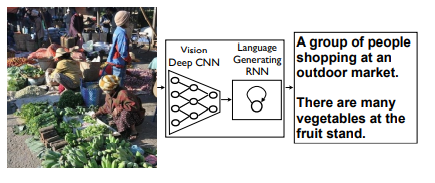
\includegraphics[width=10cm]{images/NIC_Basic_Model.png}
    \caption{NIC, our model, is based end-to-end on a neural network consisting of a vision CNN followed by a language-generating RNN. It generates complete sentences in natural language from an input image, as shown in the above example.}
    \label{fig:}
\end{figure}

In this paper the encoder RNN is replaced by a CNN, over the last few years it is shown that CNNs can produce a rich representation of the input image by embedding it to a fixed-length vector, such that this representation can be used for a variety of vision tasks. This forms the basis to use a CNN as an image "encoder", by the first pre-training it for image classification and the last hidden layer as an input to the RNN decoder that generates the sentences. This model is called Neural Image Caption (NIC) and is shown in the above figure.

\section{Related works}
\label{related works}
As the task of machine translation exist for many years there were many approaches to implement it in our everyday life. The idea of combining natural language processing and computer vision led us to the possibility of generating novel descriptions for the images.

The first ideas of combining these two areas of research appeared in the last century. The challenging task was to provide not only the list of objects on the video and their tasks but also an ensemble behaviour of all of them.  Thus, one of the works was aimed at the possibility of introducing a description of the ensemble behaviour of objects in real time. Traffic jam videos were chosen as the research object. The algorithm clearly separated stationary and dynamic motion, and also provided a behaviour characteristic of a certain group of objects from the video.

Another important part of the model is the structure of the generated sentence. Here the challenging task is to create grammatically correct, intelligible descriptions. In [2] researchers provide us with a well-described sentence formation that underlines many models today. The final description includes information about objects (or/and stuff), their description (attributes) and the spatial relationship (preposition) of objects to each other and has the structure: object/stuff description + spatial representation (object – preposition – object). Additionally, templates for linguistic constraints were applied to address correct grammar challenges.

With the development of neural networks and their success in object detection and speech recognition as well as in NLP, the idea of using this approach to solve the task of description generation of the image became quite popular. Along with this, a lot of works appeared, that combined pictures and their corresponding descriptive sentences in one space for training the algorithm.

Firstly, the images and sentences are processed separately. The next step is to combine the feature vector that represents an image and corresponding reference sentences together in one multimodal embedded space. In paper [3] the dataset that contains 5 independently created descriptions of each image were used. The idea is to train the model, to have a high inner product with related sentence vectors to the image and to have a low inner product with incorrect pairs. To optimize an algorithm the ranking cost function can be used [3,5]. The alternative cost function can be a squared loss that calculates the distances, as well as maximizes the likelihood probability of the correct description. [our paper].

Previous works have shown good results in this area in relation to the relevant capabilities of their times. Moreover, many ideas are borrowed from these works, which are used in modern models. However, all previously listed methods are limited by the fact that they are not able to properly process the pictures that have not been seen before. This can lead either to misclassification or to an error in the algorithm. Nowadays methods are aimed at solving this question.

One of the common model structures that became quite popular in neural machine translation is based on the encoder-decoder. Here, neural networks are used as a complete end-to-end translation system. In addition, certain works have shown that the process of sentence formation in machine translation can be simplified many times by using recurrent neural networks (RNNs) and still show successful results. The current work was inspired by the success of these achievements. [our paper]

In the paper [4] researchers were using RNNs autoencoder to translate phrases from English into French. The model is consist of two recurrent neural networks (RNNs):
 \begin{enumerate}
 \item Encoder: RNN encodes a sequence of symbols in a vector of fixed length;
 \item Decoder: RNN decodes fixed vector in another sequence of symbols;
 \item Hidden unit: LSTM, which decides which information to store and which can be ignored. It also can control the amount of information that is carried from the previous hidden state to the current one. As a result, we have a more compact representation of information;
 \end{enumerate}
After the training, the model can be used in both directions. On the one hand, it can generate the target sequence from the input. On another hand, it can estimate the ‘score’ of the input-output, which is simply a probability. Moreover, the algorithms were able to generate phrases that do not overlap completely with the target sentences.[4]

Since we use the image as an input, the encoder part was replaced with a convolution neural network and uses a similar approach described in [3] to train the model. But still, RNN is preferable for sentence generation.

However, the deeper the neural network is constructed, the more the problem of vanishing and exploding gradients arises. To deal with it, the LSTM, which is another form of RNN, can be used as in [5]. The idea is similar to that used in [4] as a hidden unit but to the whole decoder part. To predict the next word, the combination of image and the context of previously generated words are used. [our paper, 5].

Lastly, [6] uses an approach that is very similar to the current proposal that will be described in Section \ref{Architecture}. The difference is that NIC uses a more powerful RNN, that has direct access to the image since it was provided to its input. That significantly improved the final result of the model. [our paper]

\section{Architecture}
\label{Architecture}

Oriol et. al~\cite{NIC}, suggests a neural and probabilistic framework to generate descriptions for images. They have achieved state-of-the-art results for a powerful sequence model by maximizing the probability of the correct translation given an end-to-end input sequence. Applicable for both training and inference.

A recurrent neural network encodes the variable length input into a fixed dimensional vector and uses this representation to “decode” it to the desired output sentence. Hence, the reference paper~\cite{NIC} uses the same principle of translating the image(instead of an input sentence in the source language) to its description.

For an image the probability of the correct description was maximized directly with the formula:
\[ \theta^{*} =\;  arg\; max_{\theta} \sum_{(I,S)}\; log\; p(S|I; \theta) \label{eq:equation1} \tag{1} \]
 $\theta$ = parameters of our model,
\textit{I} is an image,
S = correct transcription of the image.
The length of S is unbounded, as it could be any sentence.
Therefore the chain rule is applicable to model the joint probability over \textit{$S_{0}$,\ldots,$S_{N}$} where \textit{N} is the length of this particular example as
\[ log p(S|I) = \sum_{t=0}^{N}log\; p(S_{t}|I,S_{0},...,S_{t-1}) \label{eq:equation2} \tag{2} \]
This equation is not dependent on $\theta$ anymore.
Further, stochastic gradient descent is used to optimize the sum of log probabilities as described in (\ref{eq:equation1}) over the whole training set on a training example pair(S, I) at training time.

 In order to model $p(S_{t}|I, S_{0},..., S_{t-1})$  with a Recurrent Neural Network (RNN), a fixed length hidden state or memory $h_{t}$ is used to express a variable number of words that is conditioned upon up to t-1. Every time the memory is updated by using a non-linear function f after a new input is visible $x_{t}$, where f is:
 \[
 h_{t+1} = f(h_{t}, x_{t}) \label{eq:equation3} \tag{3} \]

The design choice of form of f and how the images and words are fed to input $x_{t}$ is essential. Therefore, an alternative is made to use a res net that has shown state-of-the-art performance on sequence tasks like translation, i.e. LSTM(Long-Short Term Memory) net for f.
Now, comes the critical part, the representation of an image, for which CNN(Convolutional Neural Network) is chosen.
CNN has been the best choice for studying image tasks, and state-of-the-art for objection recognition and detection~\cite{NIC}.
The research paper has used CNN with a novel approach to batch normalization and it has yielded the best performance on the ILSVRC 2014 classification competition~\cite{12}. Also, It has been shown to generalize scene classification by means of transfer learning~\cite{4}. The embedding model represents the word.

\subsection{LSTM-based Sentence Generator}
\begin{figure}[ht]
    \centering
    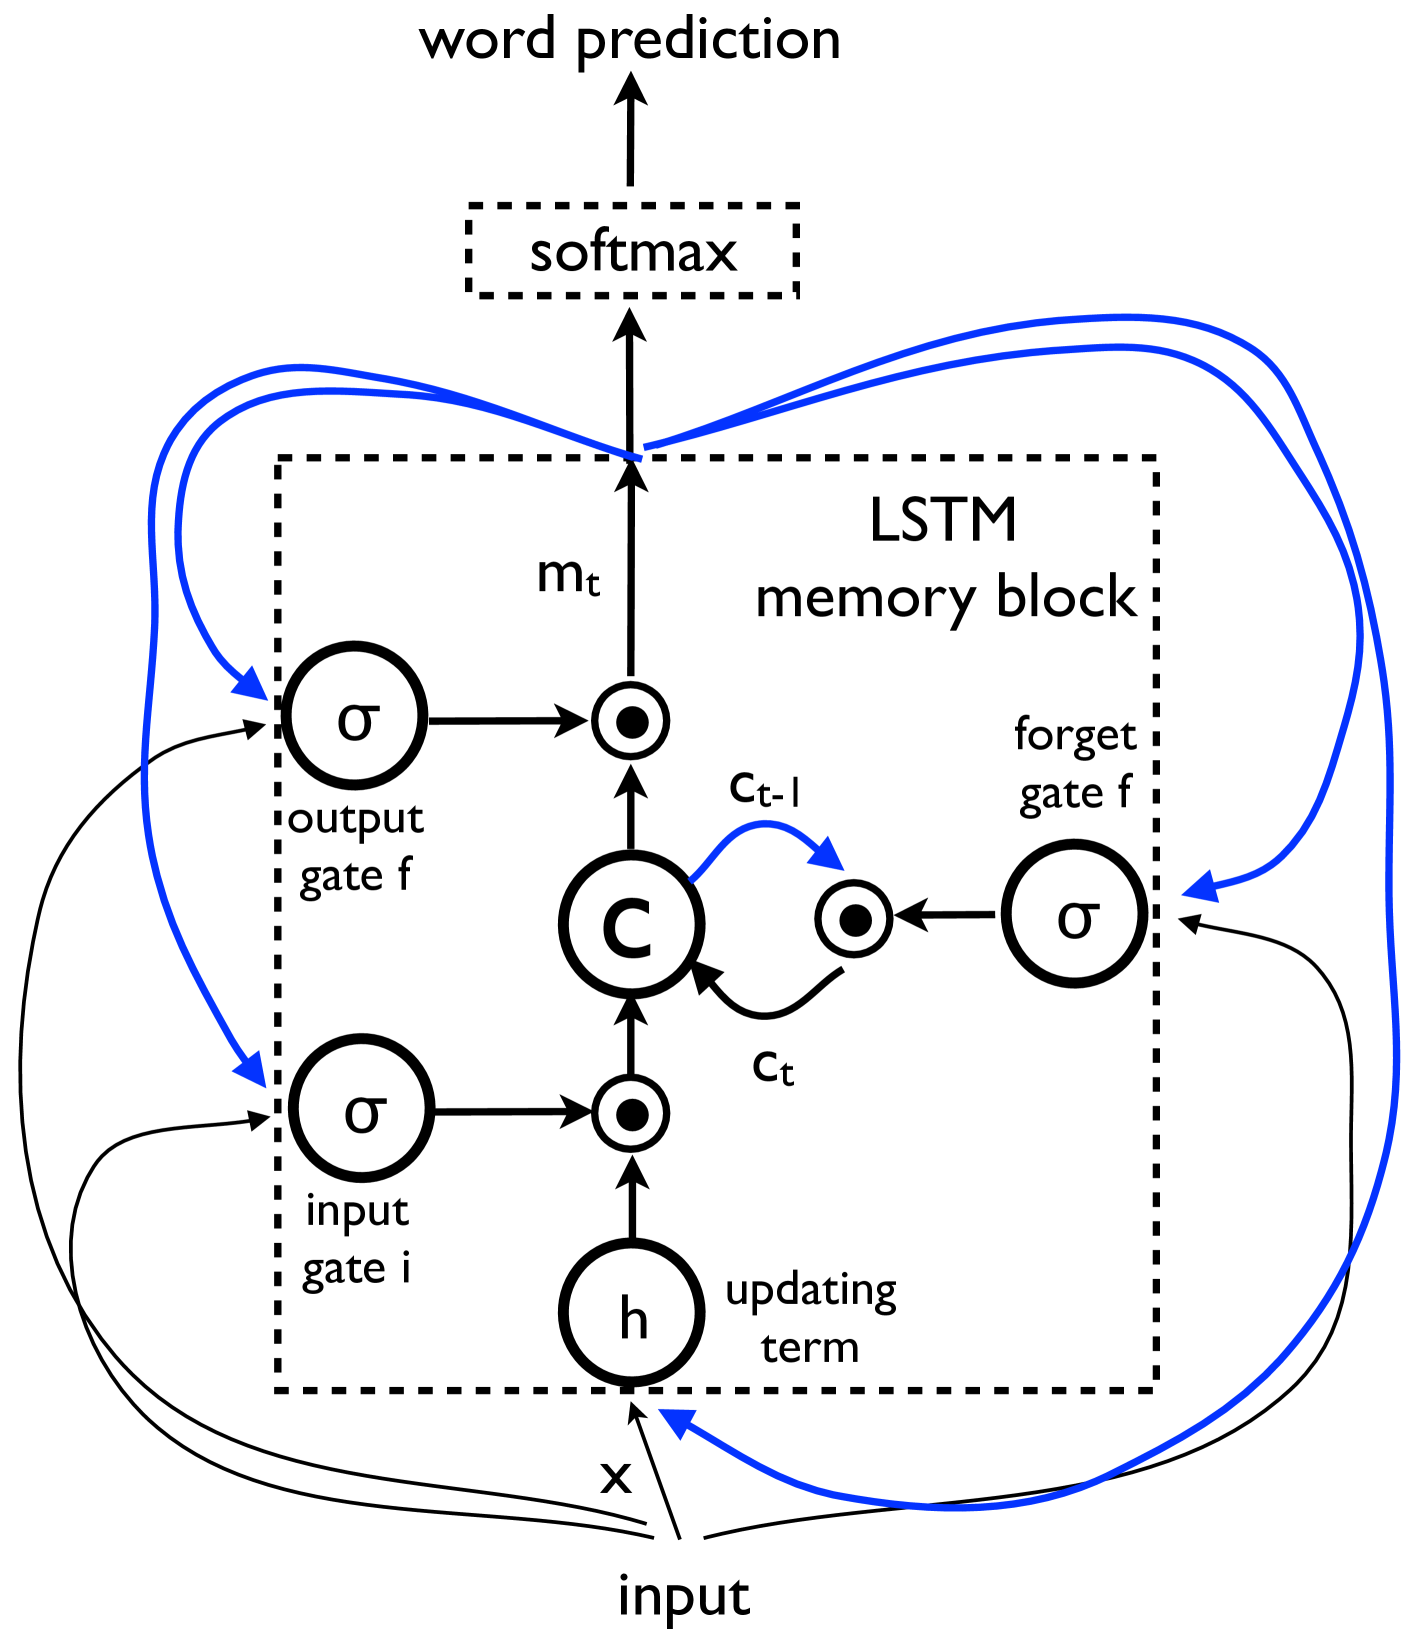
\includegraphics[width=8cm]{images/softmax lstm.png}
    \caption{ LSTM: the memory block contains a cell c which is controlled by three gates. In blue we show the recurrent connections – the output m at time t-1 is fed back to the memory at time t via the three gates; the cell value is fed back via the forget gate; the predicted word at time t-1 is fed back in addition to the memory output m at time t into the Softmax for word prediction~\cite{NIC}.}
    \label{fig:LSTM}
\end{figure}
While designing and training RNNs, the most common challenge is vanishing and exploding gradients~\cite{10} and the choice of f(\ref{eq:equation3}) is based on the ability to deal with these challenges.

As mentioned in the above section, LSTM has succeeded in translation~\cite{3} and sequence generation~\cite{9}, it also addresses the above challenge of RNNs.
The model of LSTM includes a memory cell c that encodes knowledge at every time step of what inputs have been observed up to this step as shown in the figure. The cell's behaviour is controlled by the gates.
The gates(layers) are applied multiplicatively. So it keeps the value from the gated layer if the gate is 1 or forgets if the gate is 0.
The model uses three gates to control based on the choice, if the current cell value has to be forgotten (forget gate f), if it should read its input(input gate i), and whether to output the new cell value (output gate o).
The below equations describe the gates, cell update and output:
\[ i_{t} = \sigma (W_{ix}x_{t} + W_{im}m_{t-1})  \label{eq:equation4} \tag{4} \]
\[ f_{t} = \sigma (W_{fx}x_{t} + W_{fm}m_{t-1})  \label{eq:equation5} \tag{5} \]
\[ o_{t} = \sigma (W_{ox}x_{t} + W_{om}m_{t-1})   \label{eq:equation6} \tag{6} \]
\[ c_{t} = f_{t} \odot c_{t-1} + i_{t} \odot h(W_{cx}x_{t} + W_{cm}m_{t-1}) \label{eq:equation7} \tag{7} \]
\[m_{t} = o_{t} \odot c_{t} \label{eq:equation8} \tag{8}\]
\[p_{t+1} = Softmax(m_t)  \label{eq:equation9} \tag{9} \]
where $ \odot$ represents the product with a gate value, and the various W matrices are trained parameters.
As these multiplicative gates work well against exploding and vanishing gradients, it is possible to train the LSTM.
There are also non-linearities like a sigmoid and hyperbolic tangent.
To produce a probability distribution pt over all words last equation $m_{t}$ is fed  to the Softmax.

\textbf{Training}

As defined by $p(S_{t}|I, S_{0},..., S_{t-1})$, after seeing the images and all preceding words, LSTM predicts each word of the sentence.
\begin{figure}[ht]
    \centering
    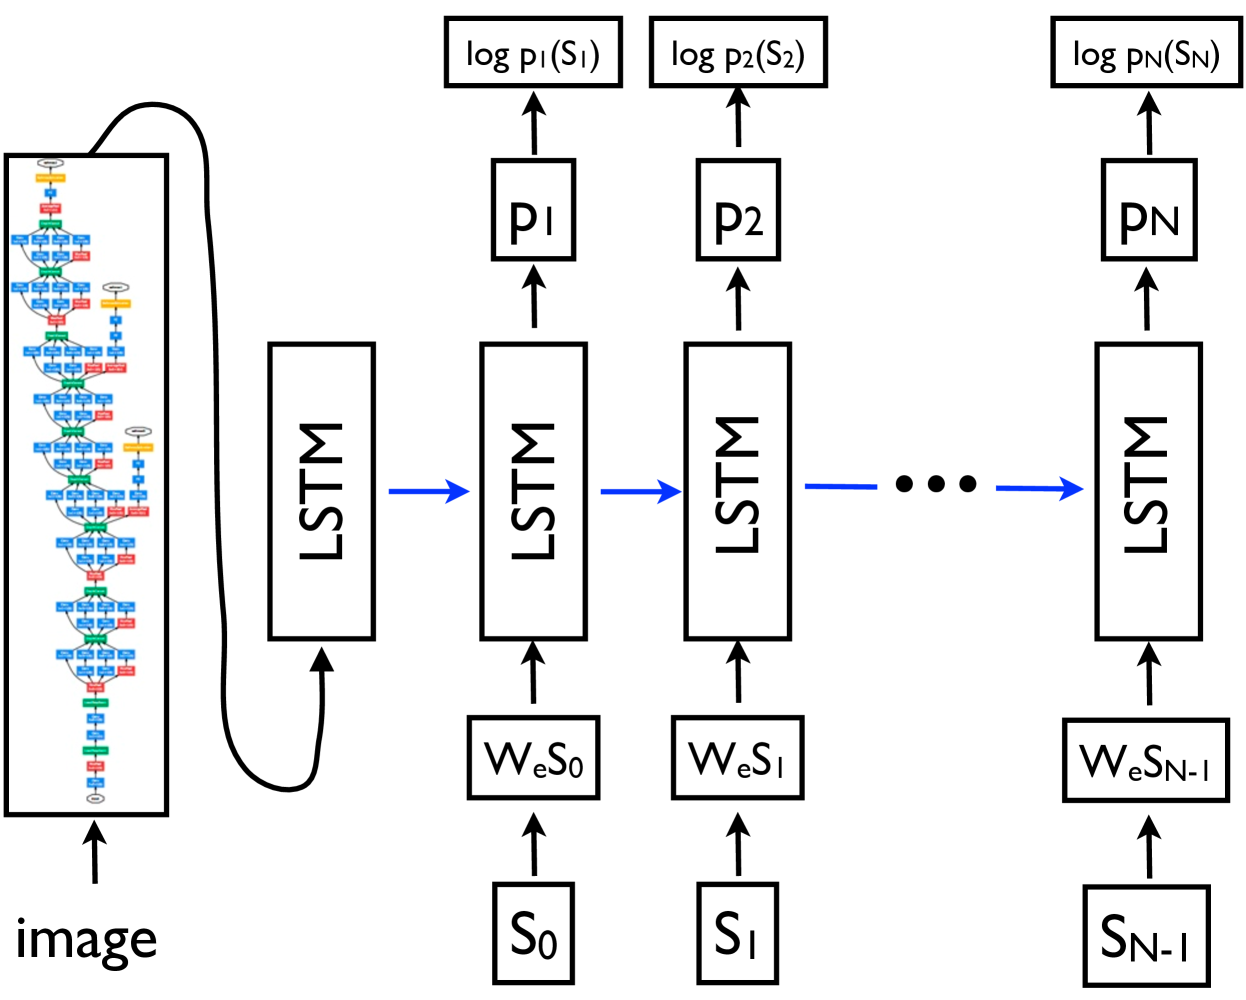
\includegraphics[width=8cm]{images/lstm.png}
    \caption{ LSTM model combined with a CNN image embedder
(as defined in ~\cite{12}) and word embeddings. The unrolled connections between the LSTM memories are in blue and they correspond to the recurrent connections in Figure \ref{fig:LSTM}. All LSTMs share
the same parameters. ~\cite{NIC}.}
    \label{fig:LSTM+CNN}
\end{figure}

As shown in figure \ref{fig:LSTM+CNN} all LSTMs share the same parameters and the output $m_{t-1}$ of the LSTM at time t-1 is fed to the LSTM at time t, therefore a copy of the LSTM memory is created for the images and each sentence word. Then all recurrent connections are transformed into feed-forward connections in the unrolled version.
If I denotes the input image and $S = (S_{0}, . . . , S_{N} )$ a true sentence describing this image,
Then
\[ x_{-1} = CNN(I) \label{eq:equation10} \tag{10} \]
\[ x_{t} = W_{e}S_{t},\; t \in {0 . . . N-1} \label{eq:equation11} \tag{11}\]
\[ p_{t+1} = LSTM(x_{t}),\; t \in {0 . . . N-1} \label{eq:equation12} \tag{12}
\]

we use $S_{t}$ of dimension equal to the size of the dictionary to represent each word as a one-hot vector.
To tell the start and end of the sentence we used $S_{0}$ a special start word and $S_{N}$ a special stop word. By emitting $S_{N}$ a special stop word we signal the LSTM that a completed sentence has been generated.
We use the same space to map the image by using a vision CNN and the words by using a word embedding We.
At t=-1, only once input is given as Image I to inform the LSTM about the image contents.

We do not feed the image at each step as an extra input as it hampers the results badly which is empirically verified, as the network exploits noise in the image and overfits more easily.

The below equation describes loss as the sum of the negative log-likelihood of the correct word at each step:
\[ L(I,S) = -\sum_{t-1}^{N} log\; p_{t}(S_{t})
\label{eq:equation13} \tag{13} \]

With respect to all the parameters of the LSTM, the top layer of the word embeddings $W_{e}$ and image embedder CNN, the loss is minimized.

\textbf{Inference} -
We can generate sentences for an image using multiple approaches, with NIC.  The first method is Sampling, where we sample the first word according to $p_{1}$, then provide the corresponding embedding as input and sample $p_{2}$, we can continue like this until we sample the special end-of-sentence token or some maximum length.
Another method is Beamsearch, which generates sentences of size t + 1, we iteratively consider the set of the k best sentences up to time t and keep only the resulting best k of them.
It can be formulated as below equation
\[
S = arg\; max_{S'} p(S' |I)
\]

The paper uses the BeamSearch approach in the following experiments, with a beam of size 20. Using a beam size of 1 (i.e., greedy search) did degrade our results by 2 BLEU points on average

\section{Datasets}
\label{Datasets}
5 different datasets that consist of images and corresponding description sentences to each of them  in English were used.

There are two datasets that were created by the same group of people: Flickr8k and Flickr30k. Flickr30k is about 4 times bigger than Flickr8k. The description of the images is based on the same vocabulary, so there are fewer discrepancies between the reference sentences.

Unlike the MSCOCO dataset that is much bigger than Flickr40k, but since the process of the data collection was done differently it has larger mismatch.

PASCAL dataset is the one that consist of 1000 samples in test set. It was collected independently from Flickr and MSCOCO. In this case, the transfer learning was applied by using other datasets to train the model.

The largest dataset that was used is SBU. It contains 1 million samples. In comparison to all previous datasets instead of human generation description it has labels (also can be counted as a weak labeling), that initially are captions. The advantage of it is the large number of data that are available for training. However, since the vocabulary is larger and noisier, it is more difficult to process it. [our paper]

The statistics of the datasets are summarized in the following table:
\begin{table}
\centering
\begin{tabular}{ |p{3cm}||p{2cm}|p{2cm}|p{2cm}|  }
    \hline
    \centering
     & \multicolumn{3}{|c|}{size}\\
    \hline
     Dataset name & Train & Valid & Test \\
    \hline
     PASKAL   & - & - & 1000\\
     Flickr8k &  6000  & 1000 & 1000\\
     Flickr30k & 28000 & 1000 & 1000\\
     MSCOCO    & 82783 & 40504 & 40775\\
     SBU &   1M  & - & - \\
     \hline
\end{tabular}
\caption{Statistics of the datasets [our paper]}
\end {table}

\section{Evaluation Metrics}
In order to check the effectiveness of NIC several experiments were conducted using different data sets, some of the experiments used are described below.

\label{Evaluation metrics}
\subsection{Human Evaluation}
This is the most reliable but at the same time the most time-consuming experiment. As part of this, people were asked to give a subjective score on the usefulness of each description that was generated using the image.

The graders were asked to evaluate each generated sentence with a scale from 1 to 4.

To conduct this experiment, an Amazon Mechanical Turk experiment was set up. Here each image was rated by 2 people. The percentage of agreement between the workers was approximately 65 percent. In case of disagreement, the scores were averaged and the average was recorded as the score.

\subsection{BLEU}
BLEU\footnote{\url{ https://machinelearningmastery.com/calculate-bleu-score-for-text-python/}} is a standart estimation approach that is used in machine translation. The idea of it is to compare generated sentence with the references. The range of it is set to be from 0 to 1, where 0 is a perfect mismatch and 1 is a perfect match. In the paper the result of BLEU is represented in precentages, therefore, the score of this evaluation range from 0 to 100.

The approach compares n-grams in the generated sentence and reference sentences and try to match them. In example, 1-gram or unigram processes each word separately, 2-gram or a bigram processes each word pair.

In the paper the BLEU-1 score is used to estimate the final performance of the algorithms. Since the dictionary contains 5 reference sentences to every image, the generated sentence was compared to each of them and the average was taken as a final score. The model was also estimated by the BLEU-4 using the same approach of taking average as a final score.
\subsection{Ranking}


\section{Results}
NIC is data-driven and trained end-to-end, experiments were conducted using different data sets to see how these data sets along with parameters like the size of the data sets, how NIC deals with weak labels, and so on might impact the overall performance of the NIC. For this experiments on five different data sets were conducted which helped in understanding the model in depth.

\subsection{Generation Diversity Discussion}
Having trained the model to be able to give p(S|I) as the output, the immediate question is whether the model generates novel captions and whether they are diverse and precise.
\begin{figure}[ht]
    \centering
    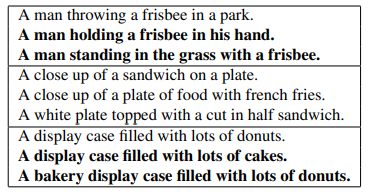
\includegraphics[width=10cm]{images/Novel_Samples.png}
    \caption{N-best examples from the MSCOCO test set. Bold lines indicate a novel sentence not present in the training set.}
    \label{fig:}
\end{figure}

The table in Figure 4 shows the N-best list extracted using the NIC model. We can notice that the samples are diverse and may also show different aspects of the same image.

In bold are the sentences that are not present in the training set. If we take the best candidate, the sentence is present in the training set 80 percent of the time. This is expected since the amount of training data is quite small, so it is easy for the model to pick "exemplar" sentences and use them to generate descriptions.

The top 15 generated sentences are analyzed and it is noticed that about half of the time there is a complete novel description. Also, the BLEU score is similar indicating that they are of enough quality and still they are quite diverse and precise.

\subsection{Human Evaluation}
Figure 5 shows the result of human evaluations of the text descriptions provided by NIC from the given image. It is compared to a reference system along with ground truth on various data sets.
\begin{figure}[ht]
    \centering
    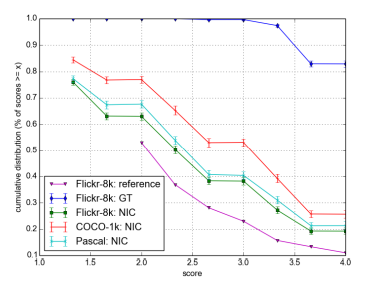
\includegraphics[width=10cm]{images/NIC_Predictions.png}
    \caption{Flickr-8k: NIC: predictions produced by NIC on the Flickr8k test set(average score: 2.37); Pascal: NIC: (average score: 2.45); COCO-1K: NIC: A subset of 1000 images from the MSCOCO test set with descriptions produced by NIC (average score: 2.72); Flickr-8k: ref: these are results from [11] on Flickr8k rated using the same protocol, as a baseline (average score: 2.08); Flickr-8k: GT: the groundtruth labels were rated from Flickr8k using the same protocol. This provides us with a "calibration" of the scores(average score: 3.89)}
    \label{fig:}
\end{figure}

\begin{figure}[ht]
    \centering
    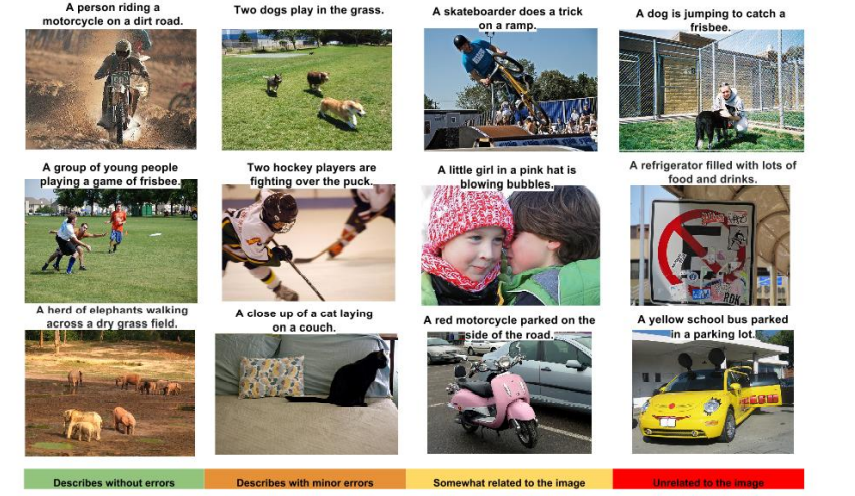
\includegraphics[width=10cm]{images/Human_Rating.png}
    \caption{A selection of evaluation results, grouped by human rating.}
    \label{fig:}
\end{figure}

NIC is better than the reference system but not as good as the groundtruth. BLEU is not a perfect metric as it fails to capture all the differences between NIC and human descriptions assessed by raters.

In Figure 6, images are rated on a scale of 1 to 4. 1 indicates that the image is well described and 4 is the worst case where the description of the image is different from what appears in the image.

The 1st column is where we have the best description of the image and in the last column, we have the case where the images described by the NIC are incorrect. It is also interesting to see, for instance in the second image of the 1st column the NIC model is able to notice the Frisbee given its size.

As observed from the above figure, this technique is quite accurate but it would be even more precise if the number of raters could be increased from 2 to say 7 or 10, which means that we have more people evaluating the description generated from the images so we would be sure that the prediction is accurate.

\subsection{BLEU}
The results of BLEU were compared with other models that also used this metric to evaluate the accuracy of the generated description, as well as with the human BLEU score. Both BLEU-1 and BLEU-4 have higher values than those for the other models. It is a bit smaller than human score, but still the closest one to it. [our paper] The results of BLEU-1 are presented in Table 2.

\begin{table}
\centering
\begin{tabular}{ |p{3cm}||p{2cm}|p{2cm}|p{2cm}|p{2cm}| }
    \hline
     \centering
     Approach & PASCAL & Flickr8k & Flickr30k & SBU \\
     \hline
     BabyTalk[] & 25 &    &    &     \\
     m-RNN[]    &    & 55 & 58 &     \\
     MNLM[]     &    & 56 & 51 &     \\
     Im2Text[]  &    &    &    & 11  \\
     \hline
     NIC[our paper] & \textbf{59} & \textbf{66} & \textbf{63} & \textbf{28}  \\
     \hline
     Human[our paper] & 69 & 68 & 70 & \\
     \hline
\end{tabular}
\caption{BLEU-1 scores [our paper]}
\end {table}


The BLEU estimation technique is inexpensive and easy to understand, that is why it is widely used in machine translation. Moreover, it doesn't depend on the language and can be used when there are more than one ground-truth. However, it does not take in account intelligibility or grammatical correctness. However, there is still the debate whether such evaluation methods are reliable and if they match human judgements. [our paper, 5]

Nonetheless, it is a subjective view how well this method corresponds to human judgments. With all the advantages of BLEU, it can be still preferable approach to estimate the final performance.
It is obvious that the description of the picture is a subjective assessment of the seen, therefore, one picture can have many possible descriptions and all of them will be correct. It should be taken into account that the number and quality of reference sentences can affect the final evaluation.

\subsection{Analysis of Embeddings}
In order to describe the image better word embedding vectors are used. The advantage is that they are independent of the size of the dictionary. These word embeddings can be jointly trained with the rest of the model.
\begin{figure}[ht]
    \centering
    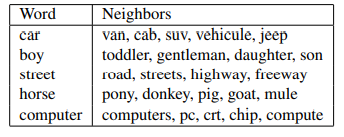
\includegraphics[width=10cm]{images/Word_Embeddings.png}
    \caption{Nearest neighbors of a few example words.}
    \label{fig:}
\end{figure}

The table in Figure 7 shows a few example words, the nearest other words found in the learned embedding space.

Some of the relationships learned by the model will help the vision component. For example, having "horse", "pony" and "donkey" close to each other will encourage CNN to extract features that are relevant to those animals that look like a horse.

It is hypothesized that in extreme cases such as "unicorn" and "horse" there is much more information provided that would otherwise be completely lost with more traditional bag-of-words-based approaches.

This is a nice feature that captures the minute details in the image and is crucial in deciding what exactly is visible in the image. For example, if we have an image where a man is driving a car, the description of the image by the NIC would be that a man is driving a car and if the man is driving a Bus, the description would be the man is driving a Bus and not the man is driving a car.
We could also add another subset that could capture more details, say for example also the brand of the automobile in the 1st row of Figure 7. The description would now be such that a man is driving a Mercedes Benz car. That is the NIC would be able to learn and predict even more detailed features with this inclusion of the new subset.

\subsection{Ranking}
\label{results}


\section{Further Improvement}
\label{further improvement}
Since one of the motivations of this idea is to help visually impaired people better understand the contents of the image. But however, if a person is completely blind he might not be able to read the text description of the image also, so we are proposing to also convert the text description into speech so that people will also be able to hear the description of the image.

More people can be involved for human evaluation, atleast 7 to 10 people might give better results.

Add novel sentences to the vocabulary. And also we can try to implement this idea using our own local images.

Try to implement the same task using unsupervised data as also proposed in this paper.

Add an image to every hidden state of LSTM to predict the next word.

Incorporate data augmentation and also check the results by changing the hyper-parameters.

Fewer data sets can be used rather than large data sets since using large data sets would need computers to have a higher computational capacity and might take several hours when normal computers are used that perform at lower speeds.


\section{Conclusion}
\label{conclusion}
In this paper NIC based approach is used to generate a reasonable description in English using images as the input to the neural network.

NIC is based on a convolution neural network (CNN) that encodes an image into a compact representation, followed by a recurrent neural network (RNN) that generates the corresponding sentence.

The model is trained to maximize the likelihood of the sentence given the image.

Several experiments have been conducted using different data sets, where we have observed that NIC performs way better than the other approaches though not as perfect as the ground truth which is expected behavior.

The BLEU score of NIC is the closest to BLEU human score.

It is also observed that as the size of the available data sets for image description increases, so will the performance of NIC. For validation and test sets, we need to have good labels.

In this paper, supervised data is used, it would also be interesting to see how unsupervised data can be used to perform the same task.












%%
%% Bibliography
%%
%bibliography file "sample.bib".

%% Please use bibtex,

\bibliography{references}

\appendix




\end{document}
